%\vspace*{1.5in}
\null

\vfill

\begin{center}
    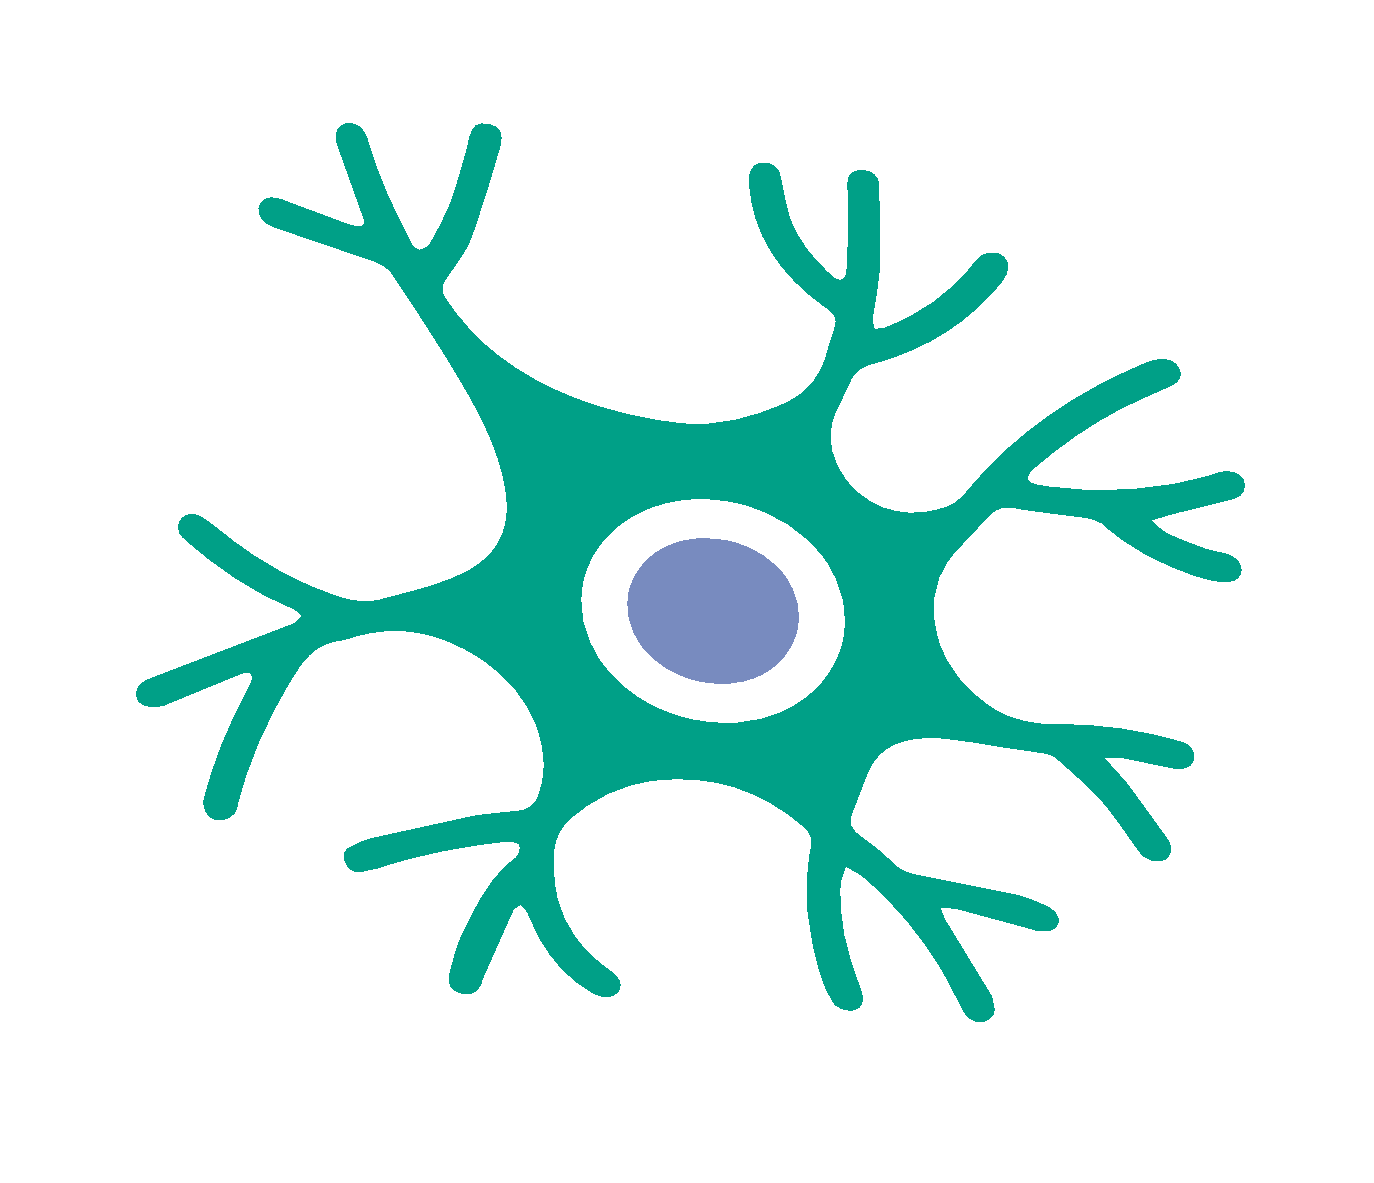
\includegraphics[width=0.3\textwidth]{src/assets/images/neuron-illustrations/neuron-illustration2.pdf}
\end{center}

\vfill

\section*{Abstract}

This thesis examines the potential of using the synchronization of oscillatory networks of PING oscillators in V1 to predict human behavior in figure-ground segregation tasks. The figure-ground segregation process, in which the brain organizes visual information into distinct objects and backgrounds, is crucial for parsing the scenes around us into meaningful objects. Previous research has suggested that the contrast and proximity of texture elements in texture stimuli affect the accuracy of figure-ground segregation. Additionally, the synchrony of neural oscillations in the gamma band is deemed to be associated with figure-ground segregation.
To explore these statements, a biologically plausible neural network of pyramidal and interneuron Izhikevich-type cells is simulated with texture stimuli that consist of Gabor annuli arranged in a grid. The stimuli vary in annuli's contrasts and grid coarseness. The synchronization of oscillations produced by the network is evaluated and compared to previously obtained behavioral data. The results show that the proposed model provides predictions of human performance in figure-ground segregation for the same stimuli. This suggests that the synchronization of oscillatory networks of PING oscillators may be a valuable predictor of figure-ground segregation.

\vspace*{1.3in}